\normaltrue
\correctionfalse

%\UPSTIidClasse{11} % 11 sup, 12 spé
%\newcommand{\UPSTIidClasse}{12}

\exer{Mouvement RT  $\star$ \label{DYN:05:B2:13:05:02}}
\setcounter{question}{0}\marginnote{\xpComp{DYN}{05}}%\UPSTIcompetence{B2-13}
\index{Compétence B2-13}\index{Compétence DYN-05}
\index{Mécanisme à 1 rotation et 1 translation}
\ifcorrection
\else
\marginnote{\textbf{Pas de corrigé pour cet exercice.}}
\fi

\ifprof
\else
Soit le mécanisme suivant. On a $\vect{AB}=\lambda(t)\vect{i_1}$.
\begin{marginfigure}
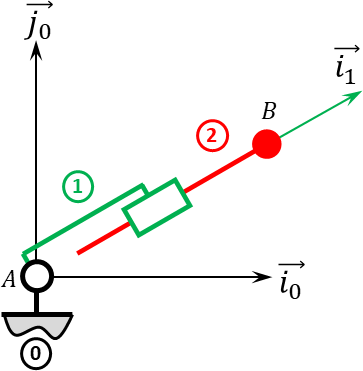
\includegraphics[width=\linewidth]{05_RT_01}
\end{marginfigure}
\fi

\question{Déterminer $\vectv{C}{2}{0}$ par dérivation vectorielle ou par composition.}
\ifprof
\else
\fi

\question{Donner le torseur cinématique $\torseurcin{V}{2}{0}$ au point $C$.}
\ifprof
\else
\fi

\question{Déterminer $\vectg{C}{2}{0}$.}
\ifprof
\else
\fi


\ifprof
\else

\marginnote{Corrigé voir \ref{DYN:05:B2:13:05:02}.}

\fi